\subsection*{Деревья решений}

Итак, на повестке дня "--- \textit{деревья решений} (\texttt{Decision trees}). Скорее всего, Вы уже прекрасно знаете, что это такое, просто не знали, как это называется. Довольно часто можно встретиться с картинками, которые объясняют их суть, да даже не это важно: размышления человека в некоторых ситуациях крайне похожи на то, что из себя представляют деревья решений.

Давайте взглянем на пример такого дерева:
\begin{figure}[H]
    \centering
    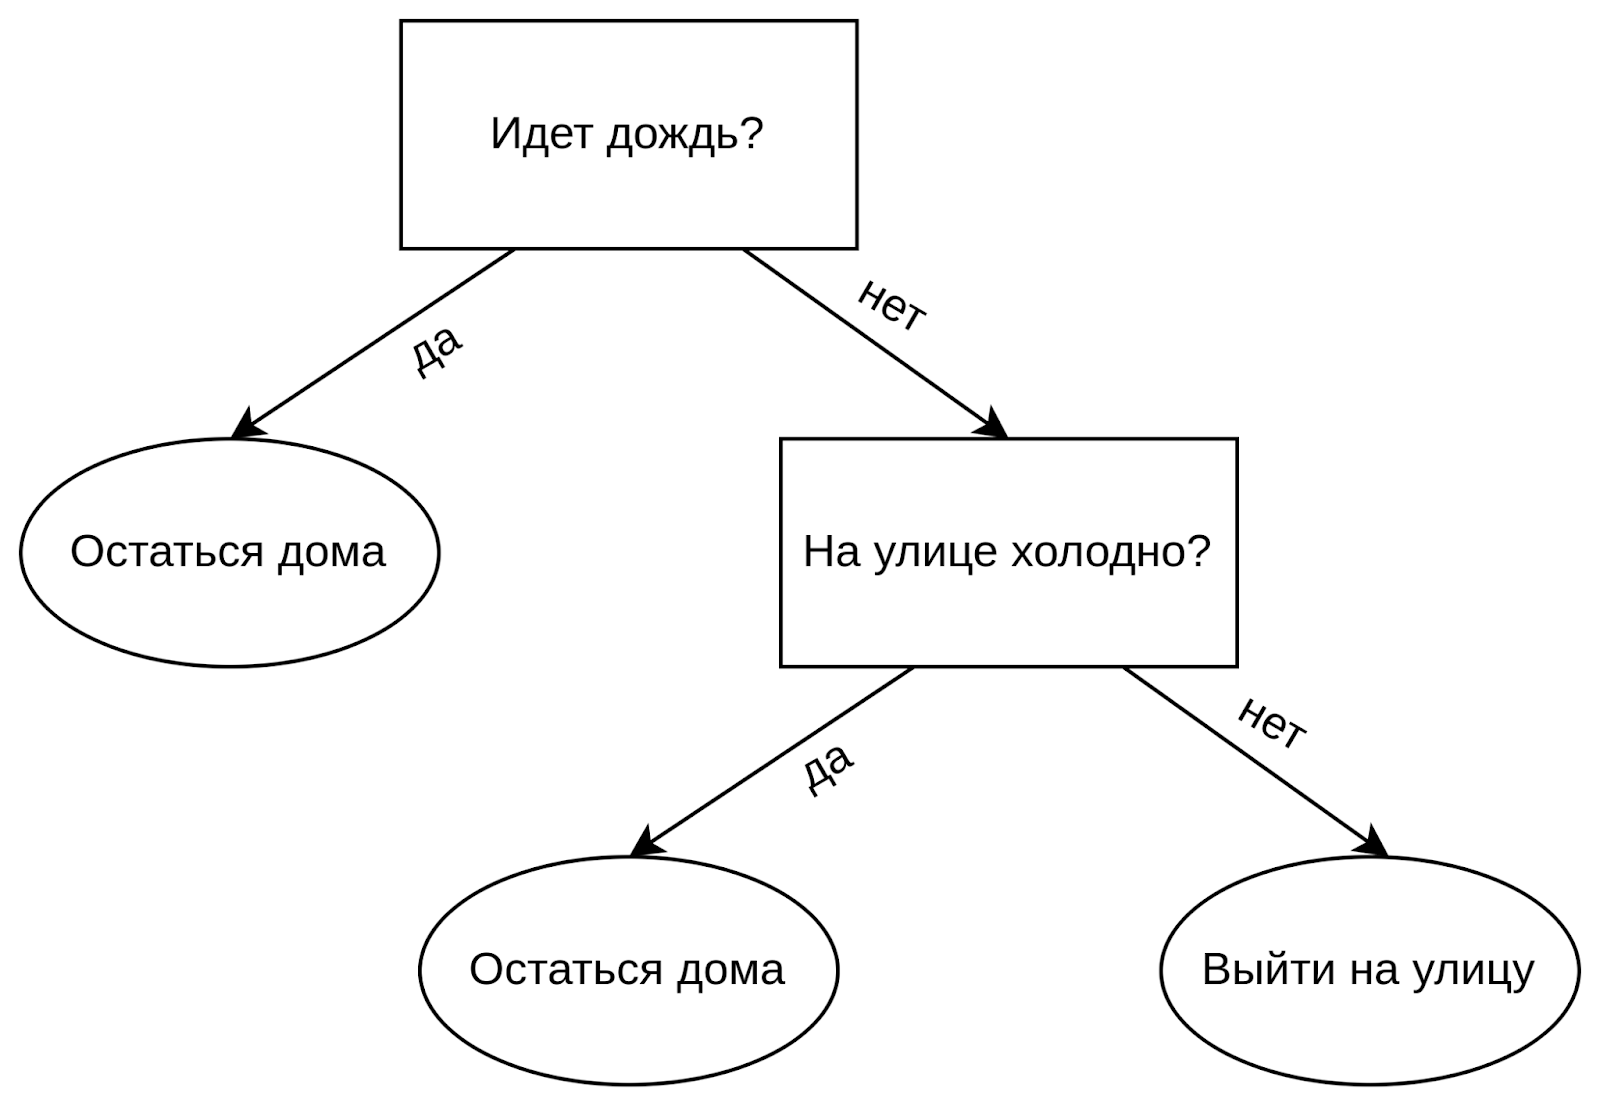
\includegraphics[width=0.75\linewidth]{img/dectree_example.png}
\end{figure}

Да, именно это из себя и представляет дерево решений! В данном случае, оно выполняет задачу классификации: на основе определённых факторов мы решаем, остаться дома или выйти на улицу. Причём просим обратить Ваше внимание на то, что необязательно опираться на какой"=то один критерий: конкретно здесь применяется и дождь, и относительная температура. Мы бы в теории могли сюда ещё добавить, например, скорость ветра, время суток и т.д.

На самом деле, деревья решений подходят как для задач классификации, так и для задач регрессии. Поэтому, говоря более формально, мы будем изучать \texttt{CART (Classification and Regression Tree)}.

\newpage

Теперь, когда мы познакомились с тем, что из себя представляют \texttt{CART}, самое время дать им более формальное определение. Решающее дерево состоит из:
\begin{itemize}
    \item Корневой узел;
    \item Ветви;
    \item Решающие (внутренние) узлы, листовые (терминальные) узлы.
\end{itemize}

Можно заметить, что это крайне похоже на бинарное дерево, и в общем случае Вы будете правы. Однако, деревья можно строить не обязательно бинарные, а значительно сложнее.

Итак, представьте что мы <<льём>> нашу выборку в это дерево сверху вниз. Корневой узел на пару с решающими узлами представляют собой некоторые <<вопросы>>, в зависимости от ответа на которые мы будем разделять поток наших объектов направо и налево. Эти вопросы мы будем называть \textit{предикатами}.

Так будет происходить до тех пор, пока объекты не достигнут терминальных узлов, которые уже будут совершать предсказание. 

В случае с линейными моделями мы предполагали, что если построить модель для двумерного случая, то модель будет являться некоторой прямой. Давайте взглянем на то, как выглядит модель дерева решений:
\begin{figure}[H]
    \centering
    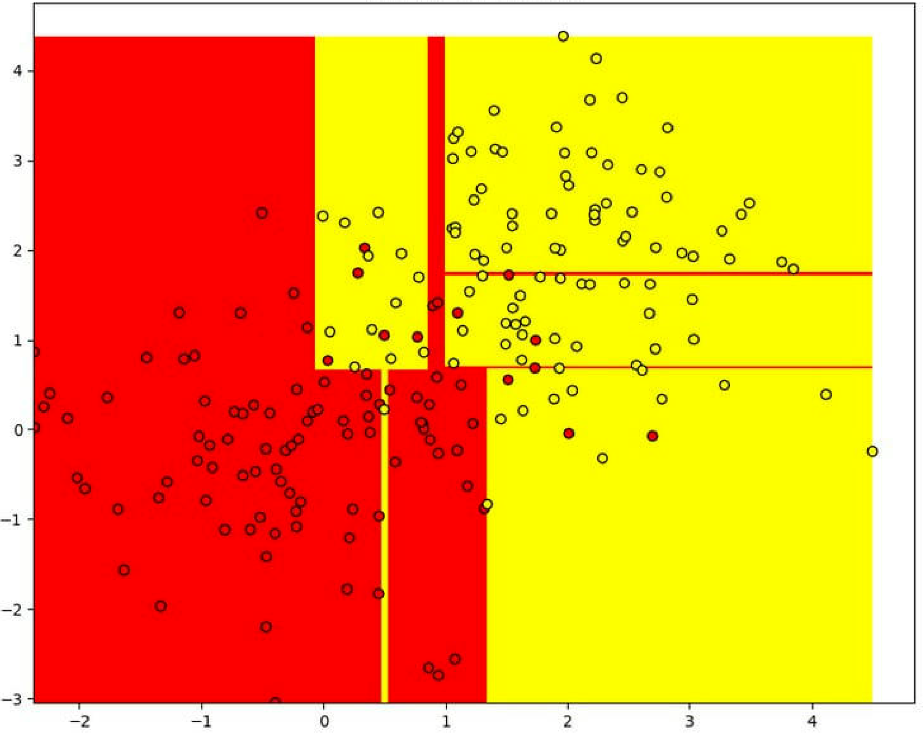
\includegraphics[width=0.75\linewidth]{img/dectree_graph.png}
\end{figure}

\newpage
Ну... давайте разбираться. Здесь изображена задача классификации, жёлтым "--- один класс, красным "--- другой класс. Дерево ставит своей задачей разбить пространство так, чтобы в каждой области лежали объекты только определённого класса. Соответствующим цветом выделена область, которая относится к классу такого же цвета (с точки зрения дерева решений). Каждый листовой узел соответствует определённой прямоугольной области на \textit{графике границ решений}.

На самом деле, можно предположить, что с помощью дерева решений можно построить классификатор, который будет идеально разбивать \textit{почти} любой случай. Это правда, однако это бессмысленно "--- дерево будет жутко переобученным, и от него будет мало толку. На рисунке в том числе можно заметить последствия переобучения: маленькие линии другого цвета среди другого класса свидетельствуют о том, что дерево намеренно построило разбиение так, чтобы захватить 1"=2 объекта из этой области.

И тут особо остро стоит вопрос, который мы уже ранее обсуждали "--- выбросы в данных. Здесь они играют более губительную роль, и уже даже в процессе построения дерева может наделать делов и окончательно сломать дерево.

Подумайте: дерево может идеально разбить почти любой случай, это мы уже обсуждали. Однако не зря выделено слово почти "--- а какой случай дерево бы не смогло разбить? (Подсказка: тут явно замешаны вероятности).